\documentclass[border=10pt]{standalone}
\usepackage{circuitikz}
\usepackage{amsmath}

\begin{document}
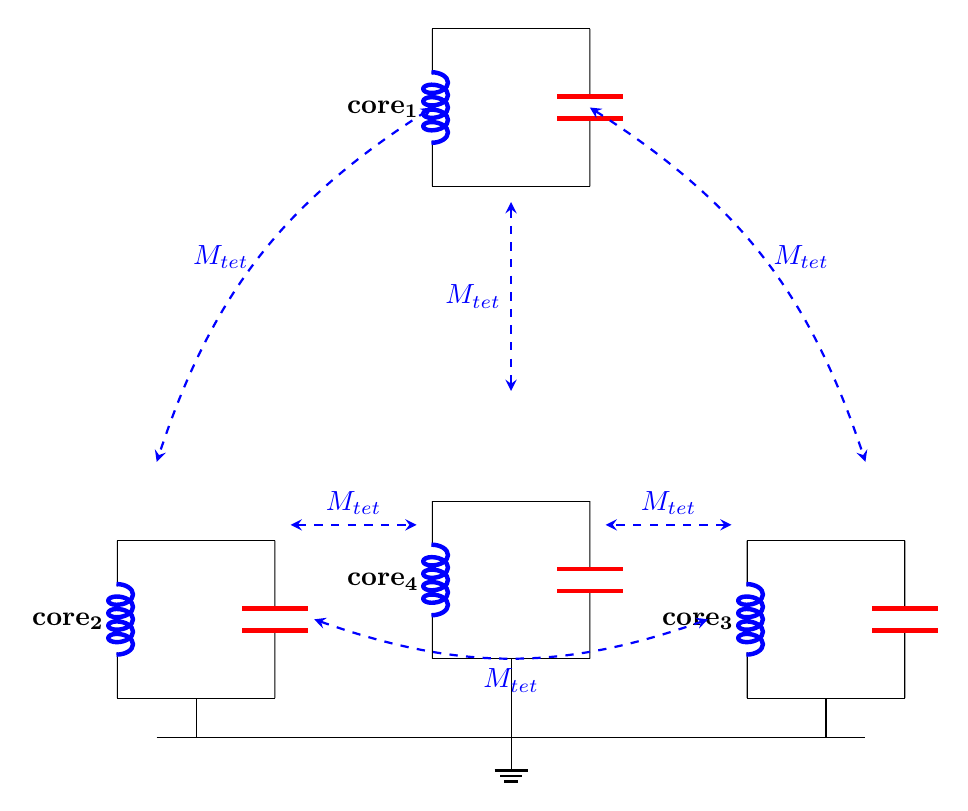
\begin{tikzpicture}

% Define macro centers for the Tetrahedron of Tetrahedrons
\def\radius{3}
\coordinate (C1) at (90:\radius);   % Top Alpha Core
\coordinate (C2) at (210:\radius);  % Bottom Left Alpha Core
\coordinate (C3) at (330:\radius);  % Bottom Right Alpha Core
\coordinate (C4) at (0,0);          % Front Central Alpha Core (Perspective)

% Function to draw an Alpha Core Tank
\newcommand{\drawalphacore}[3]{
    % #1 is the Name, #2 is the X offset, #3 is the Y offset
    \begin{scope}[shift={(#2,#3)}]
        % Draw standard LC tank for an Alpha Core (representing 4 clustered nucleons)
        \draw (-1, 0) to[L, l_=$\mathbf{#1}$, color=blue, thick] (-1, -2);
        \draw (1, 0) to[C, color=red, thick] (1, -2);
        \draw (-1, 0) -- (1, 0);
        \draw (-1, -2) -- (1, -2);
    \end{scope}
}

% Draw the four massive macroscopic bodies (Alpha Cores)
\drawalphacore{core_{1}}{0}{4.5}
\drawalphacore{core_{2}}{-4}{-2}
\drawalphacore{core_{3}}{4}{-2}
\drawalphacore{core_{4}}{0}{-1.5}

% Draw Top Level Master Ground
\draw (-4.5,-4.5) -- (4.5,-4.5);
\draw (0,-4.5) node[ground]{};
\draw (-4,-4) -- (-4,-4.5);
\draw (4,-4) -- (4,-4.5);
\draw (0,-3.5) -- (0,-4.5);

% Inter-Core Geometric Mutual Inductance (M_tet)
% Coupling C1 to C2 and C3
\draw[<->, >=stealth, dashed, thick, blue] (-1, 3.5) to[bend right=20] node[midway, left] {$M_{tet}$} (-4.5, -1);
\draw[<->, >=stealth, dashed, thick, blue] (1, 3.5) to[bend left=20] node[midway, right] {$M_{tet}$} (4.5, -1);

% Coupling C2 to C3
\draw[<->, >=stealth, dashed, thick, blue] (-2.5, -3) to[bend right=20] node[midway, below] {$M_{tet}$} (2.5, -3);

% Coupling C4 (Center) to others
\draw[<->, >=stealth, dashed, thick, blue] (0, 2.3) -- node[midway, left] {$M_{tet}$} (0, -0.1);
\draw[<->, >=stealth, dashed, thick, blue] (-2.8, -1.8) -- node[midway, above] {$M_{tet}$} (-1.2, -1.8);
\draw[<->, >=stealth, dashed, thick, blue] (2.8, -1.8) -- node[midway, above] {$M_{tet}$} (1.2, -1.8);

\end{tikzpicture}
\end{document}
